图~\ref{fig:subject-binaural-spectra}和图~\ref{fig:horizontal-error-maps}给出两名测试被试的个体重建示例。P0009按确定性规则选为“中位效应”代表：在44名测试被试中，计算每名被试相对MCA的五项比较指标改善向量，并选择与跨被试中位改善向量距离最小者。P0060作为强改善案例，用于展示被考察被试中较大的综合幅度改善。图~\ref{fig:subject-binaural-spectra}分别在左耳$270^\circ$与右耳$90^\circ$的对侧插值方向上展示结果；实测HRTF为黑色实线，MCA为灰色虚线，FSC为红色实线。

\begin{figure}[htbp]
\centering
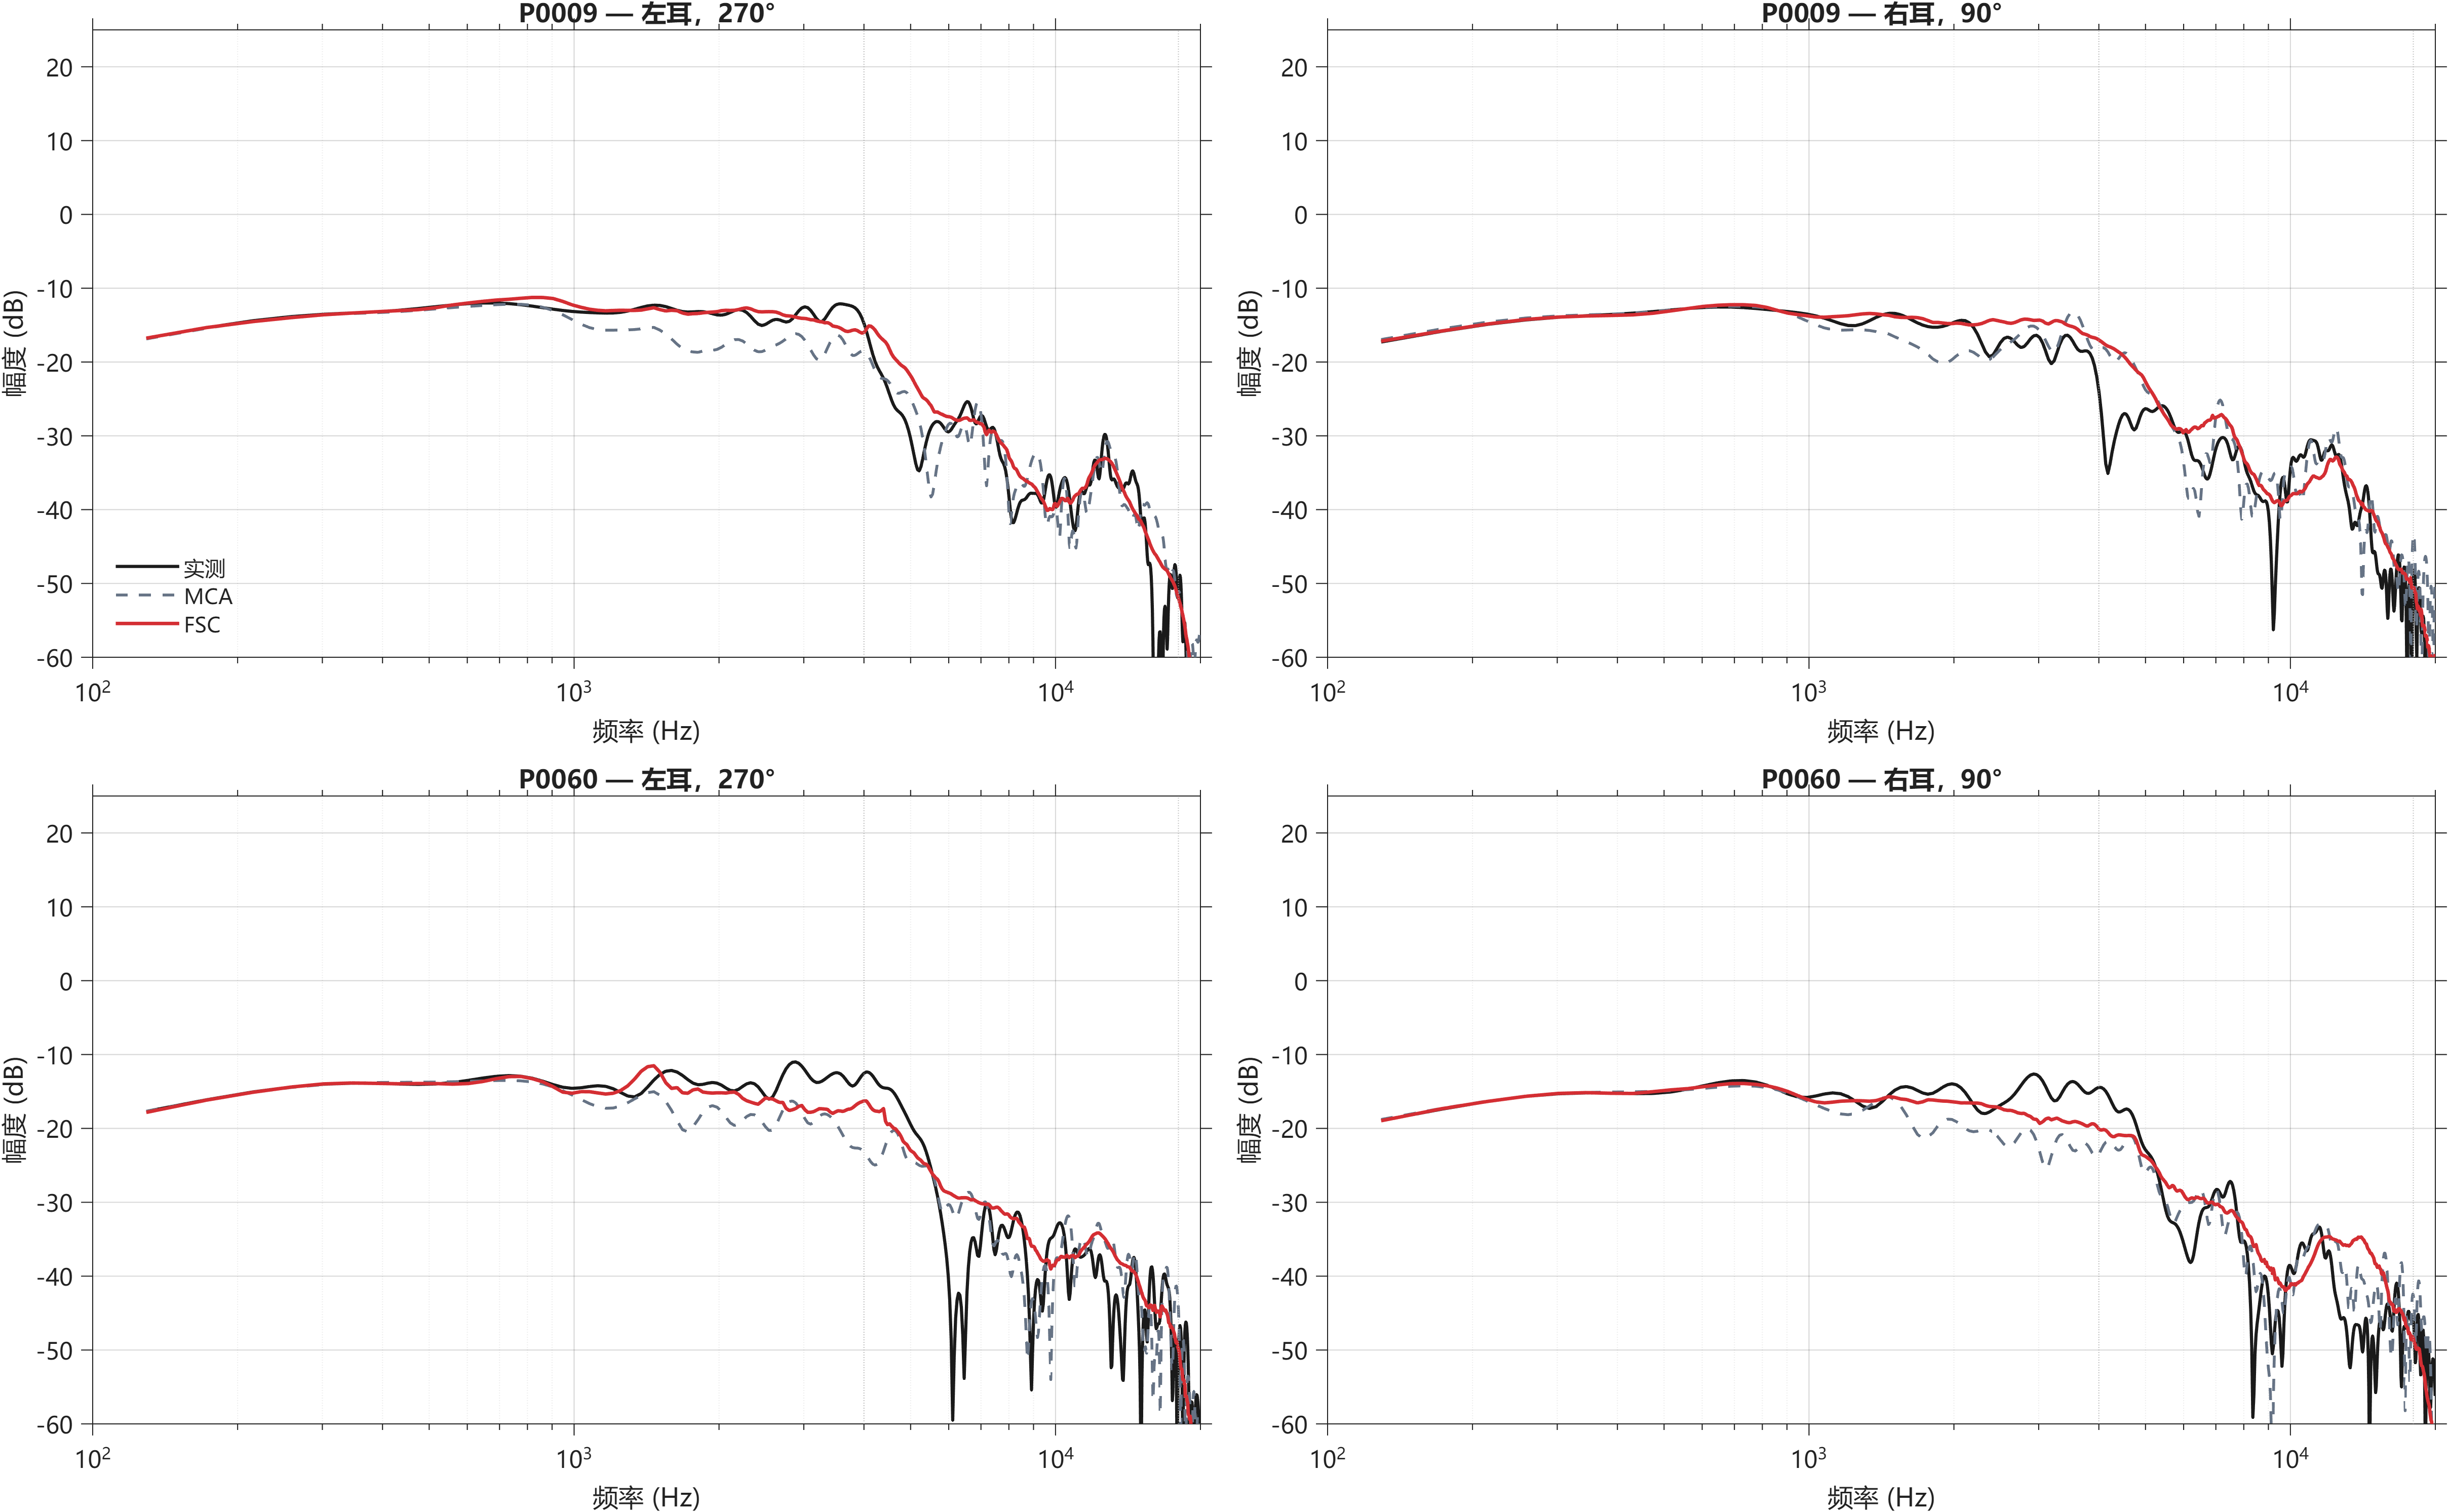
\includegraphics[width=0.98\linewidth]{figure/fsc_two_subject_binaural_spectra_zh.png}
\bicaption[fig:subject-binaural-spectra]{图}{P0009和P0060在对侧插值方向上的双耳HRTF幅度谱}{Fig.}{Binaural HRTF magnitude spectra for P0009 and P0060 at contralateral interpolation directions}
\end{figure}

在这些对侧插值方向上，FSC在较宽的中高频区域通常比MCA更接近实测幅度，但部分窄带峰值和谱凹口仍存在失配。因此，这里的校正更适合解释为对MCA残差频谱的进一步补偿，而不是对所有局部谱凹口的精确恢复。图~\ref{fig:horizontal-error-maps}进一步将比较从单个对侧查询方向扩展到全部72个水平面插值方向。对每名被试，图中依次给出实测左耳幅度、MCA绝对误差和FSC绝对误差，后两者采用统一的0--12\,dB色标。虚线标记左耳对侧方向$270^\circ$，在图示方位角坐标中等价于$-90^\circ$。从整个水平面来看，两名被试中MCA重建的多处误差脊在FSC细化后均有所减弱，尤其体现在方向相关的中高频结构上。

\begin{figure}[htbp]
\centering
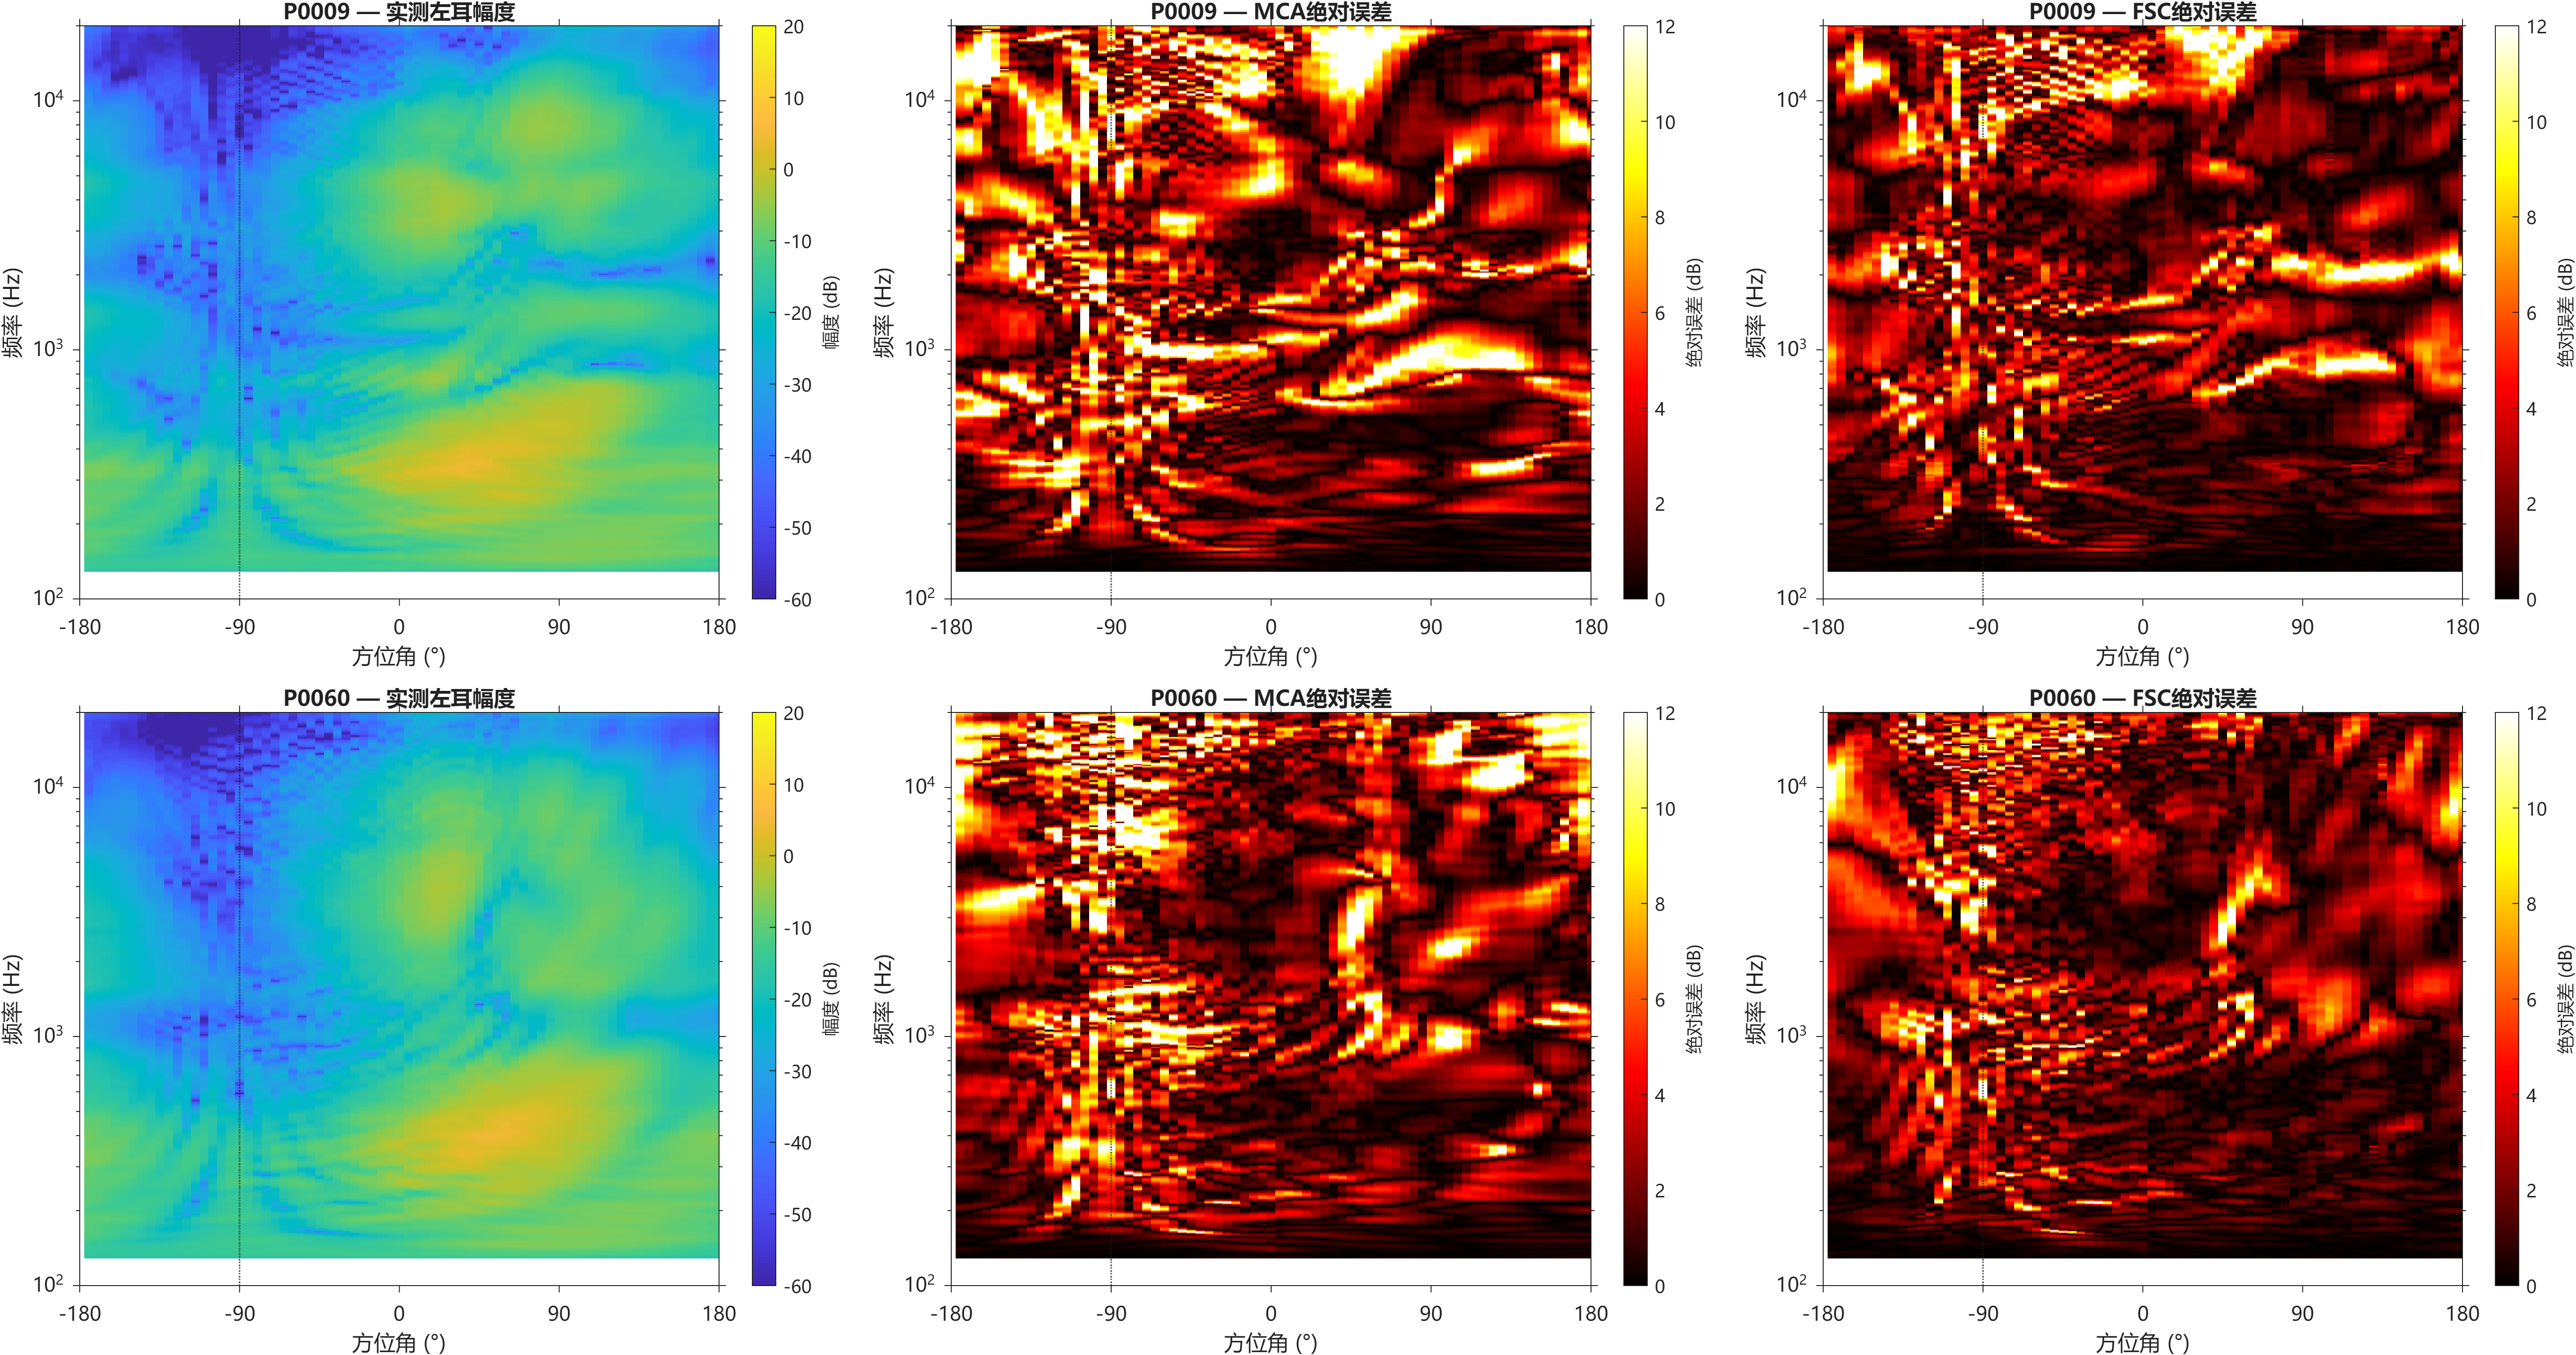
\includegraphics[width=0.98\linewidth]{figure/fsc_two_subject_horizontal_maps_zh.png}
\bicaption[fig:horizontal-error-maps]{图}{P0009和P0060的水平面左耳HRTF幅度与绝对误差图}{Fig.}{Horizontal-plane left-ear HRTF magnitude and absolute-error maps for P0009 and P0060}
\end{figure}
